\documentclass[xetex,mathserif,serif]{beamer}

% Hyperlinks.
\usepackage{hyperref}

% % Language settings.
% \usepackage{polyglossia}
% \setdefaultlanguage[babelshorthands=true]{russian}

% Setting outer theme.
\useoutertheme{infolines}

% Setting font.
\usepackage{fontspec}
\setmainfont{FreeSans}
\newfontfamily{\russianfonttt}{FreeSans}

% Code highlighting.
\usepackage[outputdir=build]{minted}
\usepackage{xcolor}

% Images.
\usepackage{graphicx}
\usepackage{animate}
\usepackage{subfig}


\usepackage{mathtools}

\title[Recommender system]{A hybrid approach \\ for news recommender system \\ using optimization methods}
\author[Alexander Smirnov]{Alexander Smirnov}
% \author[Alexander Smirnov]{Alexander Smirnov\\ \footnotesize supervisor: Elena Mikhailova}

\begin{document}


\frame{\titlepage}

% \section{Introduction}

% \subsection{Approaches}

\begin{frame}
	\frametitle{Introduction}

	\begin{itemize}
		\item Many approaches
		      \begin{itemize}
			      \item Content-based
			      \item Collaborative
		      \end{itemize}
	\end{itemize}

\end{frame}


\begin{frame}
	\frametitle{Content-based approach}

	\begin{figure}[h]
		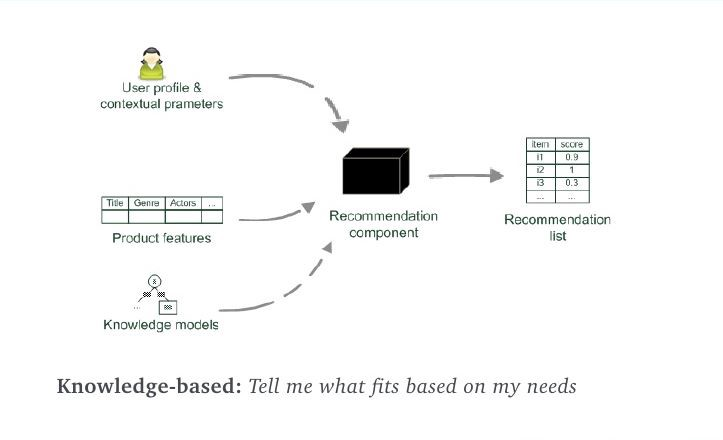
\includegraphics[width=0.9\textwidth]{./images/content_based.jpeg}
		\centering
	\end{figure}
\end{frame}


\begin{frame}
	\frametitle{Collaborative approach}

	\begin{figure}[h]
		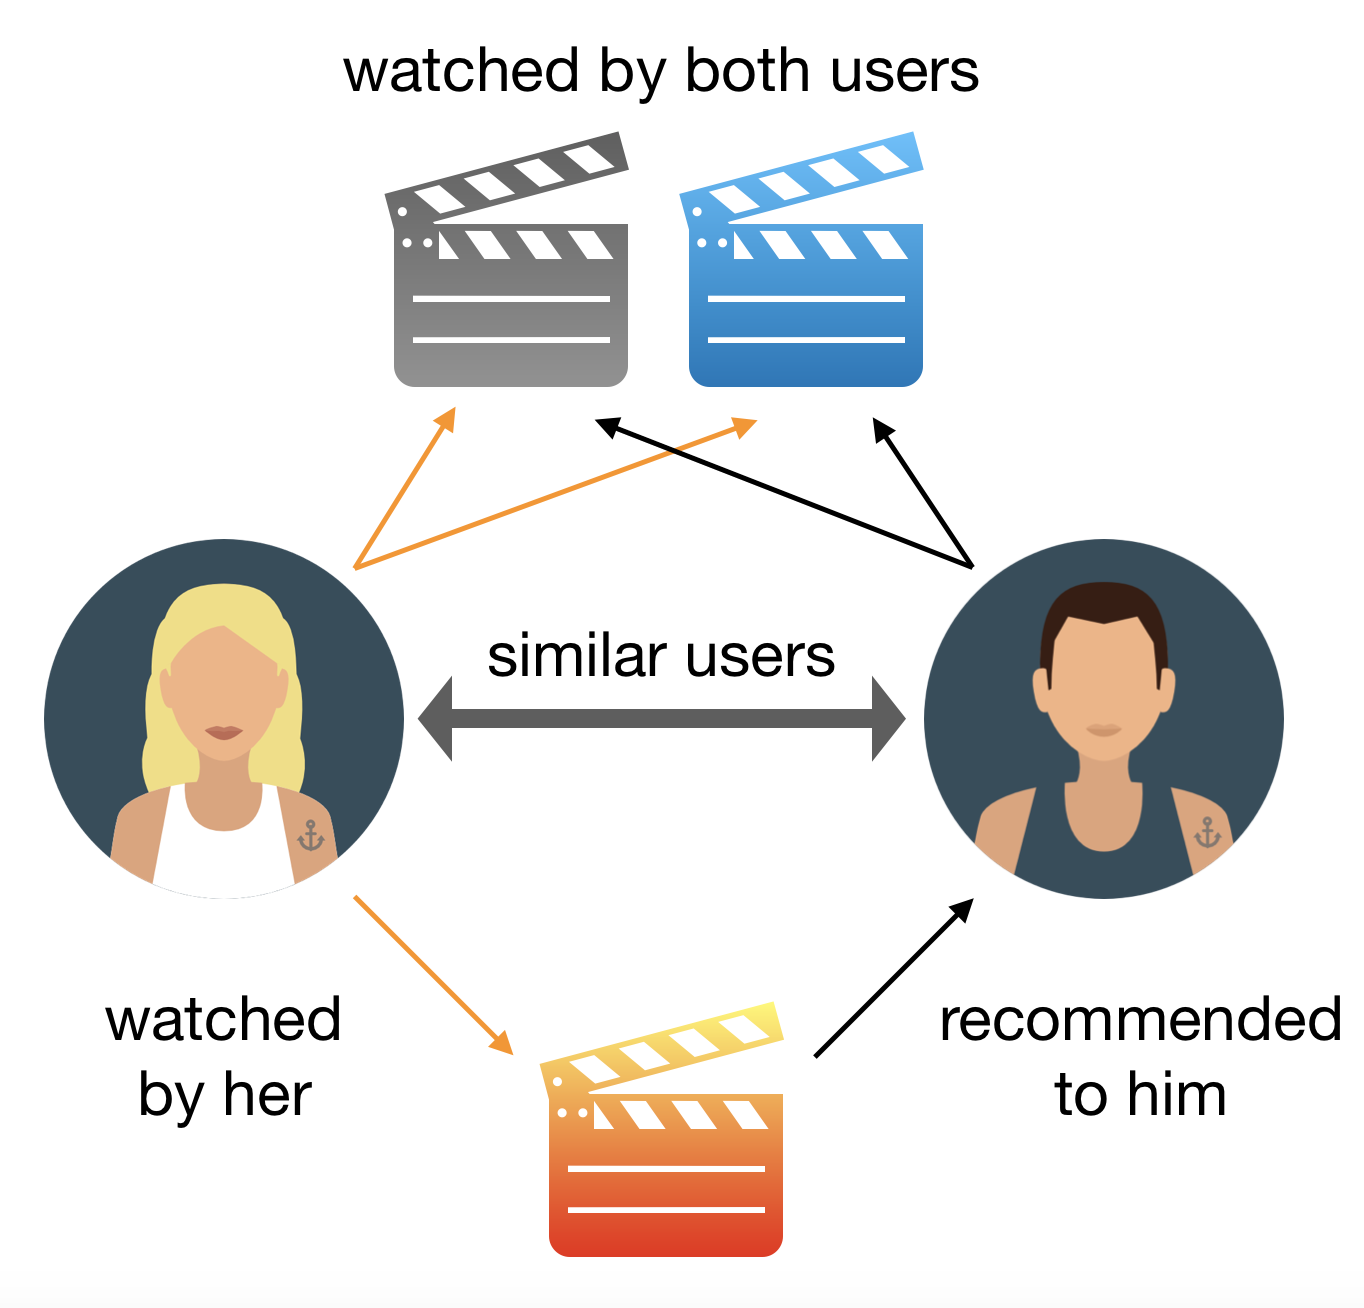
\includegraphics[width=0.5\textwidth]{./images/collaborative.png}
		\centering
	\end{figure}
\end{frame}



\begin{frame}
	\frametitle{Goal}

	\begin{itemize}
		\item Scalable hybrid news recommender system
		\item Use as many information as possible
		      \begin{itemize}
			      \item users' logs
			            \begin{itemize}
				            \item likes
				            \item comments
				            \item views
				            \item shows
				            \item etc
			            \end{itemize}
			      \item news' features
			            \begin{itemize}
				            \item source
				            \item popularity
				            \item theme
				            \item etc
			            \end{itemize}
		      \end{itemize}
	\end{itemize}
\end{frame}


\begin{frame}
	\frametitle{Solution}

	\begin{itemize}
		\item Hybrid recommender
		      \begin{itemize}
			      \item Collaborative recommender
			      \item Content-based recommender
			      \item Last Viewed recommender
			      \item Boost recommender
		      \end{itemize}
		\item Optimize weights
	\end{itemize}
\end{frame}


\begin{frame}
	\frametitle{Diagram}

	\begin{figure}[h]
		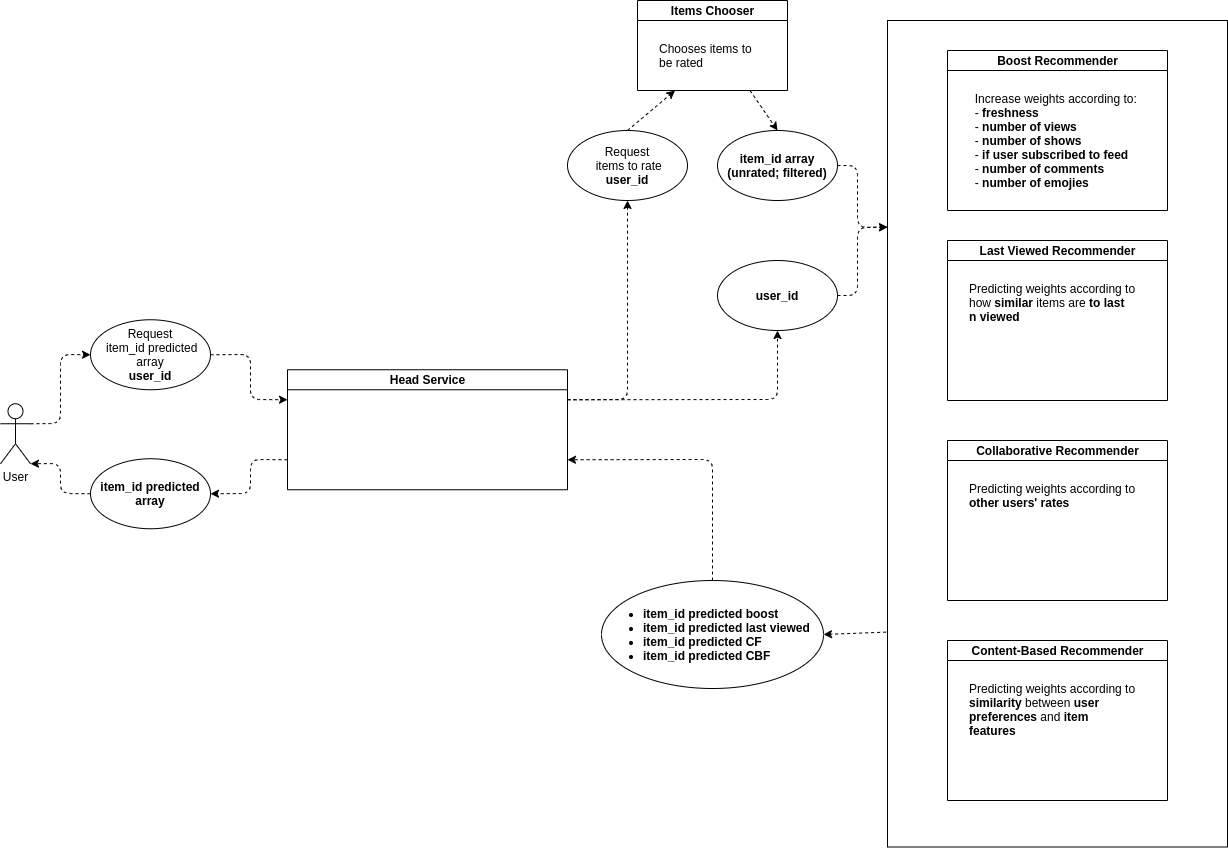
\includegraphics[width=0.8\textwidth]{./images/main.png}
		\centering
	\end{figure}
\end{frame}



\begin{frame}
	\frametitle{Difficulties}

	\begin{itemize}
		\item Many approacher to every recommender
		      \begin{itemize}
			      \item A / B testing
		      \end{itemize}
		\item Many candidates (candidate generation)
		\item High load
	\end{itemize}
\end{frame}

\end{document}
